\section{Classification methods}
\label{sec:methods}
Using the generated features, five methods wereapplied to classify the data into positive and negative classes. Three of the methods are linear classifiers that were applied to the Tweet-embedding representations. The other two are neural network-based classifiers which were directly applied on word-embeddings.

\subsection{Logistic regression}
The first classifier that is applied is standard logistic regression. This classifier use the logistic function classify the Tweets into one of two classes. The advantage of this method is that it is simple to implement, and computationally efficient. It can be used to determine if the modification of the data processing has an impact on classification.

\begin{figure}[h!]
\centering
	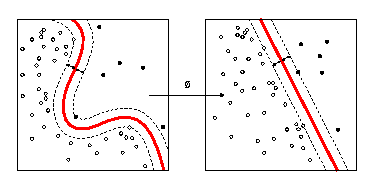
\includegraphics[scale=1.2]{SVM} 
\caption{The support vector machine draws a decision boundary between points that seeks to maximise the surrounding margin. The boundary can be linear, or another ``shape'' according to a supplied kernel function.\cite{wikiSVM}}
\label{plot:SVM}
\end{figure}
\FloatBarrier

\subsection{Support vector machine}
The support vector machine (SVM) is a more advanced linear classification model, traditionally used in supervised learning tasks. This makes it a potentially good fit for the task at hand. Given a set of training examples belonging to two different classes, the SVM model determines a boundary between examples of the two classes, then seeks to maximise the intervening margin. In addition to linear decision boundaries, the SVM can be supplied with different kernel functions that modify the shape of the boundary (see Figure \ref{plot:SVM}). In all instances, the notion of drawing a boundary and maximising the margin remains.

\subsection{Neural networks}

Neural nets were also used on tweets features. This neural net has one layers of size (200,100) . This was to take account that a neural network of  two layers is sufficient to represent any vectorial function.  If this technique was giving the best results of all the one that were used on on tweets representation, it didn't lead to the sufficiently good results for the competition. 

\subsection{Convolutional neural networks}
The convolutional neural network (CNN) extends upon the ``standard'' neural network that seeks to further exploit locality data in addition. Here, a method inspired by Yoon Kim's seminal paper was employed \cite{cnnYoon}. The notion is that exploiting positional information in the Tweet should yield more information than simply using vectorial sums of word-embeddings.
In the context of this task, each Tweet is represented by a matrix: each word in a Tweet corresponds to a row in the matrix, containing that word's embeddings. Thus, the matrix is of size $W \times D$ for $W$ words in the Tweet, and $D$ word-embedding dimensionality.
The model we implement applies a first convolution layer, and subsequently, filters of varying sizes (here, 3, 4, and 5) which are used in a sliding window fashion over the elements of the matrix. The output is then the result of a chosen activation function---here we use the rectifier linear unit (ReLU). Each convolution creates a tensor of a different size, to which a pooling process is applied, in order to subsample the different tensors into further tensors of a standard size. Finally, the standard tensors are combined to create a large feature vector, which is used to create the predictions using matrix multiplication.

\begin{figure}[h!]
\centering
	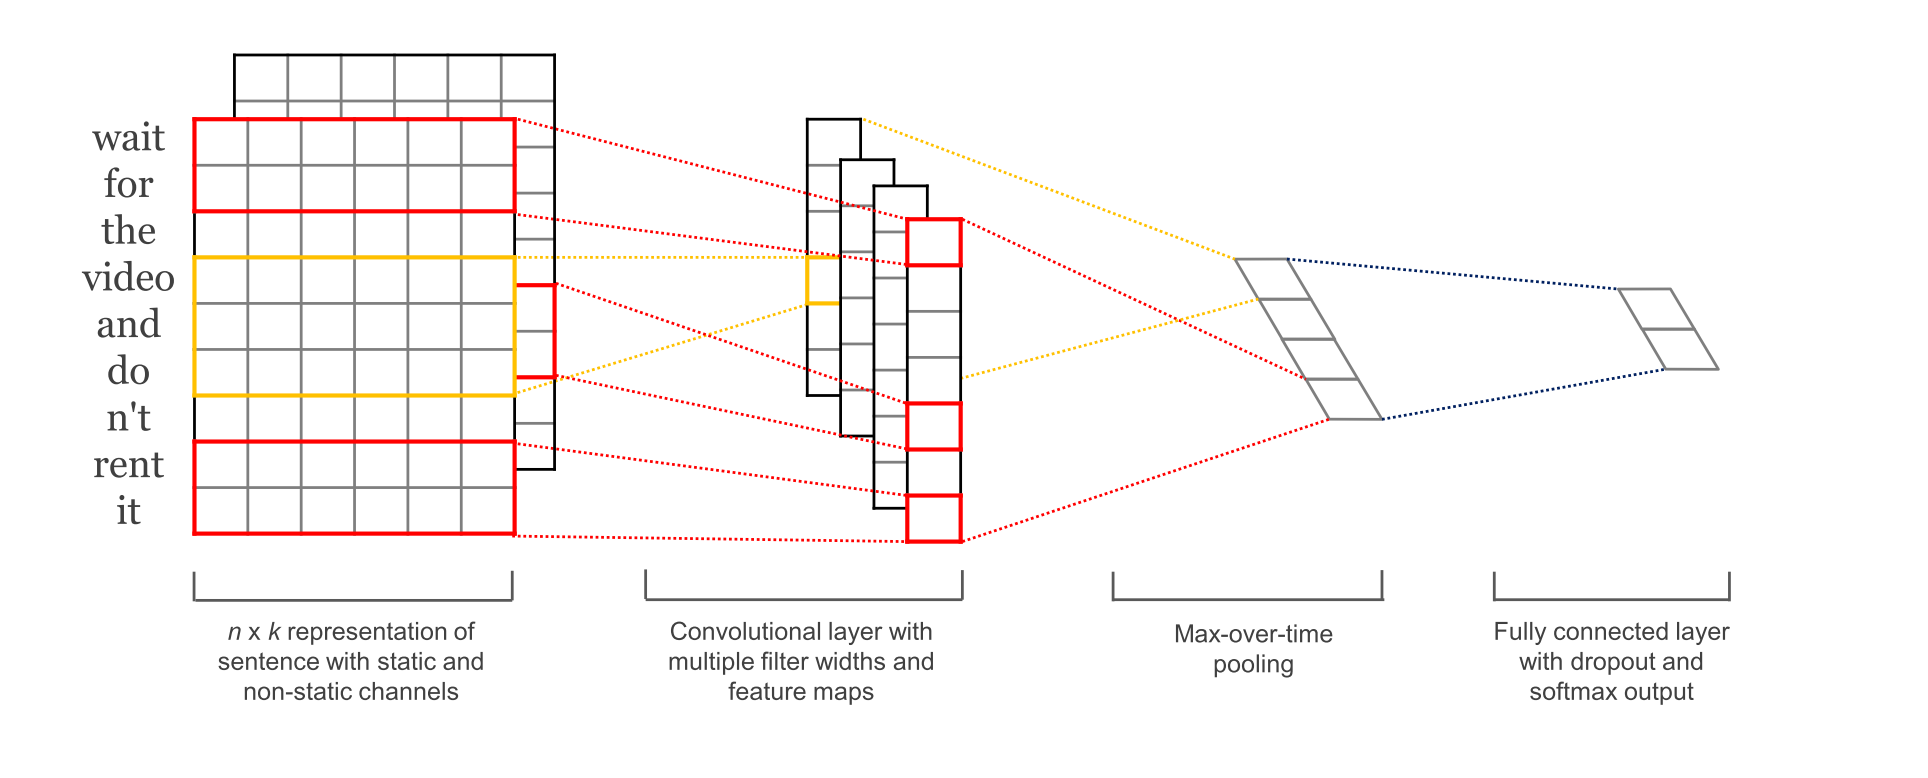
\includegraphics[scale=0.2]{CNN} 
\caption{Architecture of the convolutional neural network used for sentiment analysis \cite{cnnYoon}}
\label{plot:CNN}
\end{figure}
\FloatBarrier

\subsection{Dropout layer}
One of the most common problems in machine learning is that of overfitting. When a fully connected convolutional neural network is trained, allowing all the nodes to interact allows too much freedom for the system, and often leads to overfitting. To solve this problem, a ``dropout'' is added to the convolutional neural network. At each step of the process a node is either kept or dropped out of the model according to some given probability. The input nodes are exempt from this procedure in order to retain the most information, while addressing overfitting. When data are tested, the full network is used and all nodes are weighted according to their probability of being retained in the model.

This methods has two advantages: first, as not all nodes are trained with the entire dataset, overfitting will be reduced; second, the use of a dropout layer significantly improves the speed of the training process. This technique reduces node-to-node interactions too, and therefore leads to more robust features.
